\capitulo{1}{Introducción}

%Descripción del contenido del trabajo y del estrucutra de la memoria y del resto de materiales entregados.

El desarrollo de software es un proceso muy complejo que depende de múltiples factores: equipo de desarrollo, tipo de producto software, estabilidad de los requisitos funcionales, importancia de los requisitos no funcionales como escalabilidad, seguridad, licencias, lenguaje de programación, tipo de arquitectura de computación...

Existen varias metodologías que ayudan a definir las actividades y artefactos del proceso de desarrollo de software. Los artefactos son las salidas de las actividades y el conjunto de artefactos conforman el producto software. En el caso de  Unified Process (UP) \cite{jacobson_proceso_2000} se identifican las siguientes actividades o flujos de trabajo: recolección de requisitos, diseño e implementación, pruebas, despliegue. Además en UP se añaden tres flujos de trabajo de soporte: configuración de cambios, gestión de proyecto y entorno. Estos flujos de trabajo se aplican iterativamente durante varias fases del desarrollo en cada una de las cuales se incrementa el producto software con algun artefacto resultado de la actividad. La característica de iteración e incremental es recogida en otros métodos o buenas prácticas de desarrollo ágiles\cite{noauthor_scrum_2019}: 
Scrum,eXtreme Programming,Lean...
%\todo Añadir referencias bibliográficas a libros


Una suposición subyacente de la administración de la calidad es que la calidad del proceso de desarrollo afecta directamente a la calidad de los productos a entregar \citep[pág 543]{sommerville_ingenierisoftware_2002}.
La calidad del proceso es uno de los factores que determinan la calidad del producto software, tal y como expone Sommerville en \textit{Ingeniería de software}\cite{sommerville_ingenierisoftware_2002}.

Los repositorios de código son espacios virtuales donde los equipos de desarrollo generan los artefactos colaborativos procedentes de las actividades de un proceso de desarrollo. En los repositorios además de guardar los artefactos, version final y versiones previas, se almacena la interacción de los miembros del equipo justificando el cambio de version. Dependiendo del artefacto generado se utiliza distintos sistemas: foros de comunicación, sistemas de control de versiones, sistemas de documentación, sistemas de gestión de issues, gestión de pruebas, de revisiones de calidad, de  integración y despliegue contínuo \cite{guemes-pena_emerging_2018}.

En la última década han surgido forjas de proyectos software de fácil acceso tanto para proyectos empresariales como para proyectos open source (SourceForge \footnote{\url{https://sourceforge.net/}}, Github \footnote{\url{https://github.com/}}, GitLab \footnote{\url{https://about.gitlab.com/}}, Bitbucket  \footnote{\url{https://bitbucket.org/}}).  Estas forjas suelen integrar múltiples sistemas para dar soporte a los flujos de trabajo y registrar las interacciones entre los miembros del equipo. Además dan la posibilidad de extensión funcional con sistemas de terceros para gestionar otras actividades no soportadas directamente, por ejemplo Travis CI
\footnote{\url{https://travis-ci.org/}} para gestionar la integración contínua o Codacy \footnote{\url{https://www.codacy.com/}} para gestionar las revisiones automáticas de calidad. Actualmente estas forjas han tenido una gran aceptación entre la comunidad de desarrolladores y existen muchos desarrollos de software de tendencia que las utilizan. La forjas de proyectos software proporcionan interfaces de programación específicas que permiten acceder a toda la información registrada. 
En la Fig. \ref{fig:Mintro-trendforja} se aprecia como cambia la tendencia de utilización de dichas forjas en el tiempo. Actualmente la forja predominante es claramente GitHub pero se ve un incremento en el uso de Gitlab.

\begin{figure}[!h]
	\centering
	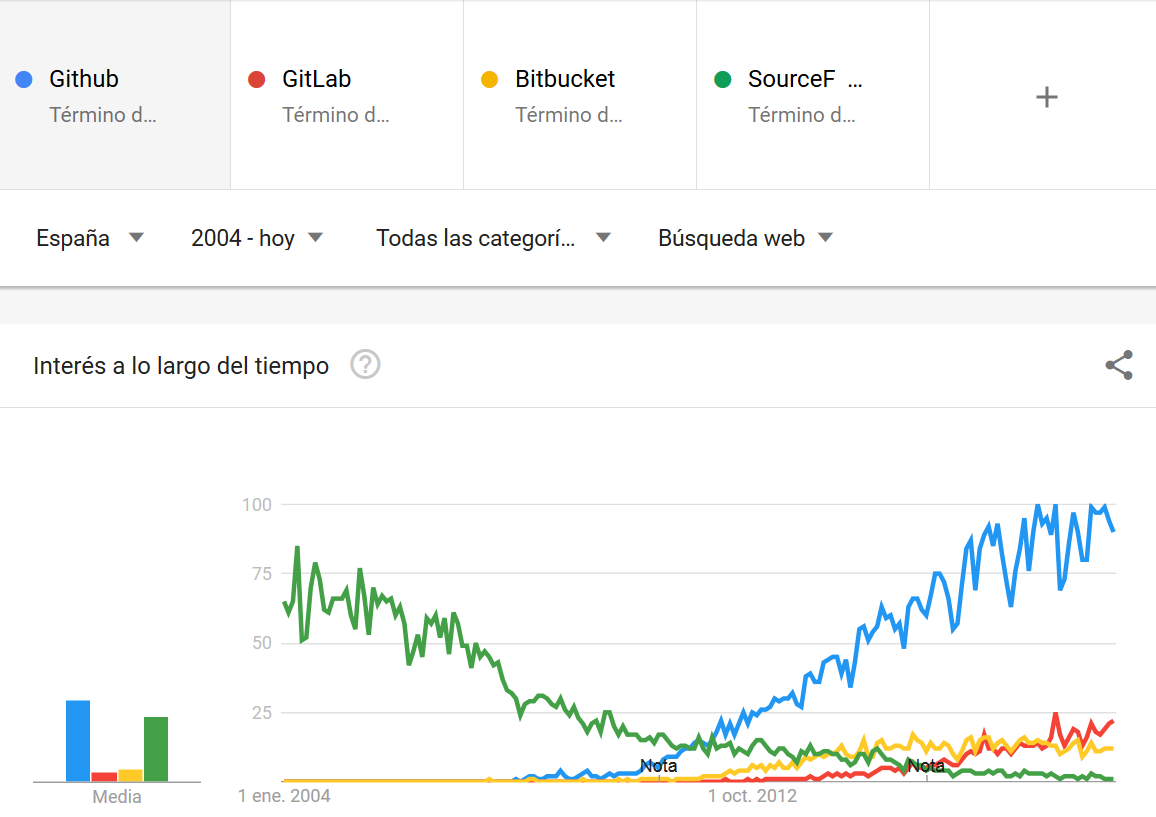
\includegraphics[scale=0.4]{Mintro-trendforja.png}
	\caption{Comparativa de tendencia de búsqueda de Google desde 2004 con los términos de distintas forjas de proyectos software.}
	\label{fig:Mintro-trendforja}
\end{figure}



 
Parece lógico considerar como hipótesis que la calidad de un artefacto software tenga alguna relación con la manera en la que el equipo  aplica las actividades del proceso de desarrollo dentro del repositorio.  
La validación empírica de estas  hipótesis ha abierto una nueva línea de aplicación con los conjuntos de datos extraídos de los repositorios.  
Estas forjas de proyectos software están en constante evolución, tanto en sus estructuras estáticas como en sus interacciones dinámicas en los proyectos. Se registran grandes conjuntos de datos difíciles de procesar. El  desafío a la comunidad científica y empresarial  es constante mostrando un incremento en el interés en las aplicaciones que mejoren sus sistemas de decisión.

Este trabajo presenta el diseño y desarrollo de una aplicación Java Web que: calcula un conjunto de métricas de evolución del proceso,
 de proyectos software alojados en GitLab, para posteriormente, compararlos en relación con otros proyectos.

\section{Estructura de la memoria}

La memoria se estructura de la siguiente manera\footnote{\url{https://github.com/ubutfgm/plantillaLatex}}\cite{ubu_plantilla_2019}:

\begin{description}
	\tightlist
	\item[Introducción.] Introducción al trabajo realizado, estructura de la memoria y listado de materiales adjuntos.
	\item[Objetivos del proyecto.] Objetivos que se persiguen alcanzar con la realización del proyecto.
	\item[Conceptos teóricos.] Conceptos clave para comprender los objetivos, el proceso y el producto del proyecto.
	\item[Técnicas y herramientas.] Técnicas y herramientas utilizadas durante el desarrollo del proyecto.
	\item[Aspectos relevantes del desarrollo.] Aspectos destacables durante el proceso de desarrollo del proyecto.
	\item[Trabajos relacionados.] Otros proyectos de la misma naturaleza y los cuales han ayudado a la realización de este.
	\item[Conclusiones y líneas de trabajo futuras.] Conclusiones tras la realización del proyecto y posibilidades de mejora o expansión.
\end{description}

Se incluyen también los siguientes anexos:

\begin{description}
	\tightlist
	\item[Plan del proyecto software.] Planificación temporal y estudio de la viabilidad del proyecto.
	\item[Especificación de requisitos del software.] Análisis de los requisitos.
	\item[Especificación de diseño.] Diseño de los datos, diseño procedimental y diseño arquitectónico.
	\item[Manual del programador.] Aspectos relevantes del código fuente.
	\item[Manual de usuario.] Manual de uso para usuarios que utilicen la aplicación.
\end{description}